\newsavebox{\HGgraphicbox}
\begingroup
\makeatletter
\let\HGoriginalendfloatbox\@endfloatbox
\def\@endfloatbox{\HGoriginalendfloatbox
  \typeout{HG-FLOAT-HEIGHT=\the\ht\@currbox}
  \typeout{HG-FLOAT-DEPTH=\the\dp\@currbox}}
\makeatother
\begin{figure*}[t]
  \centering
  \sbox{\HGgraphicbox}{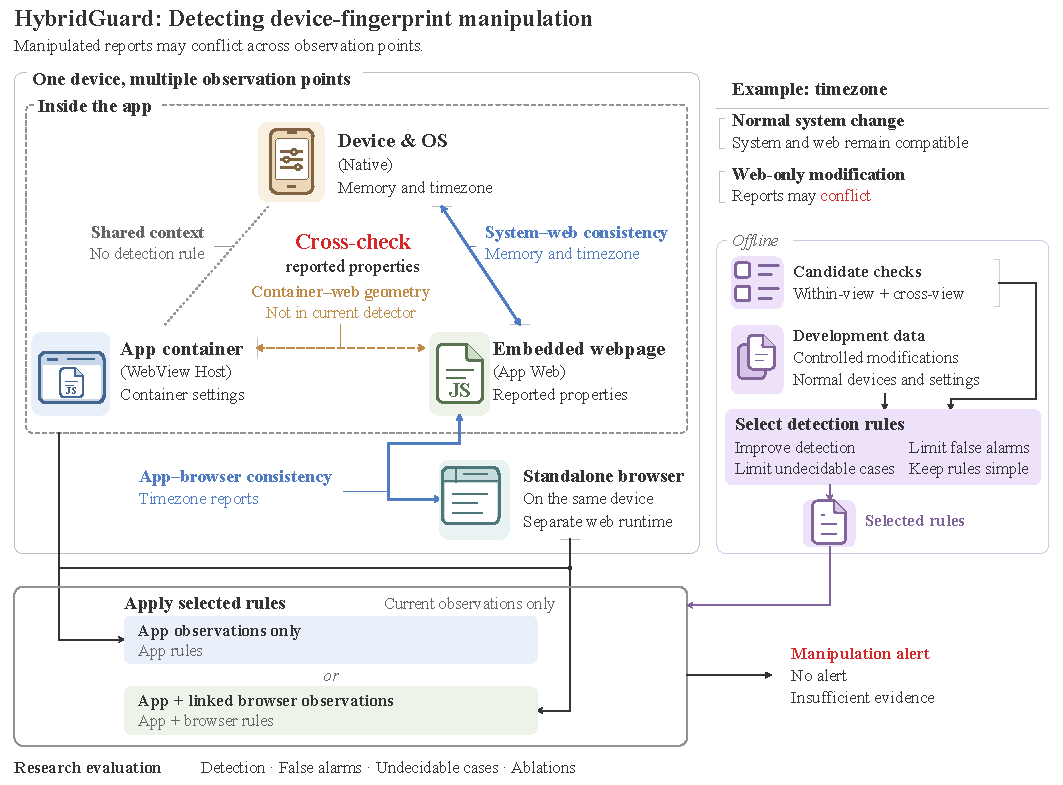
\includegraphics[width=\textwidth]{figures/HybridGuard_overview_candidate.pdf}}
  \typeout{HG-TEXTWIDTH=\the\textwidth}
  \typeout{HG-TEXTHEIGHT=\the\textheight}
  \typeout{HG-GRAPHIC-WIDTH=\the\wd\HGgraphicbox}
  \typeout{HG-GRAPHIC-HEIGHT=\the\ht\HGgraphicbox}
  \typeout{HG-GRAPHIC-DEPTH=\the\dp\HGgraphicbox}
  \typeout{HG-BODY-FONT=\fontname\font}
  \usebox{\HGgraphicbox}
  \caption{HybridGuard checks device-fingerprint reports for possible manipulation using complementary observations from the same device. Within-view and cross-view checks are evaluated on controlled modifications and normal operation to select compact detection rules under false-alarm and decision-coverage constraints. The selected detectors process current App observations alone or linked App--browser observations and return a manipulation alert, no alert, or insufficient evidence. The inset illustrates why changing a system setting need not have the same cross-view effect as modifying only a webpage's report. Solid comparison edges indicate relations used in the detectors; Host--web geometry remains a separate study, and the dotted Native--Host link denotes context only. No observation point is trusted ground truth. No alert does not establish safety. Execution failures are recorded separately.}
  \Description{Device and OS, app container, and embedded webpage form a triangle inside one app. A standalone browser lies outside the app, on the same device. Solid system--web and app--browser comparisons are selected; dashed container--web geometry is not in the current detector, and the dotted Native--Host edge is context only. Two independent timezone illustrations explain compatibility and possible conflict. Offline candidate checks and development data lead to selected rules. Current App-only and linked App--browser observations enter vertically stacked alternative modes marked or, using their corresponding fixed rules. A separate model port loads selected rules into the common application frame. One arrow from that frame leads to the selected mode's result list; there is no result fusion. Research evaluation is a separate scope strip.}
  \label{fig:hybridguard-overview}
\end{figure*}
\endgroup
